%----------------------------------------------------------------------------------------
%    PACKAGES AND THEMES
%----------------------------------------------------------------------------------------
\documentclass[aspectratio=169,xcolor=dvipsnames]{beamer}
\makeatletter
\def\input@path{{../BeamerTemplate/theme/}}
\makeatother
\usetheme{CleanEasy}
\usepackage[utf8]{inputenc}
\usepackage{lmodern}
\usepackage[T1]{fontenc}
\usepackage{fix-cm}
\usepackage{amsmath}
\usepackage{mathtools}
\usepackage{listings}
\usepackage{xcolor}
\usepackage{hyperref}
\usepackage{graphicx}
\usepackage{booktabs}
\usepackage{tikz}
\usetikzlibrary{positioning, shapes, arrows, calc, decorations.pathreplacing, arrows.meta, backgrounds, patterns, overlay-beamer-styles}
\usepackage{etoolbox}

%----------------------------------------------------------------------------------------
%    LAYOUT CONFIGURATION
%----------------------------------------------------------------------------------------
\input{../BeamerTemplate/configs/configs}

%----------------------------------------------------------------------------------------
%    TITLE PAGE CONFIGURATION
%----------------------------------------------------------------------------------------
\title[Introduction to DS]{Introduction to Data Structures}
\author{Data Structure Course}
\institute{DGIST}
\date{\today}

% Simple title page without logos
\titlegraphic{}

%----------------------------------------------------------------------------------------

\begin{document}

\begin{frame}[plain]
  \titlepage
\end{frame}

\begin{frame}[plain]{Contents}
  \tableofcontents
\end{frame}

%----------------------------------------------------------------------------------------
%    DEFINITION AND ROLE
%----------------------------------------------------------------------------------------
\section{What Are Data Structures?}

\begin{frame}{Definition}
  \begin{definition}
    A \textbf{data structure} is a specialized format for organizing, storing, and managing data in a computer so that it can be accessed and modified efficiently.
  \end{definition}

  \vspace{0.5cm}

  \begin{columns}
    \begin{column}{0.48\textwidth}
      \textbf{Why We Need Them:}
      \begin{enumerate}
        \item \textbf{Efficiency} \\
              Right structure = milliseconds \\
              Wrong structure = hours
        \item \textbf{Organization} \\
              Systematic data management
        \item \textbf{Reusability} \\
              Solve similar problems
        \item \textbf{Abstraction} \\
              Hide implementation details
      \end{enumerate}
    \end{column}
    \begin{column}{0.48\textwidth}
      \begin{exampleblock}{Real-World Analogies}
        \begin{itemize}
          \item \textbf{Bookshelf} $\rightarrow$ Array \\
                {\small Organized for easy retrieval}
          \item \textbf{Filing cabinet} $\rightarrow$ Hash table \\
                {\small Labeled drawers}
          \item \textbf{Stack of plates} $\rightarrow$ Stack \\
                {\small Take from top}
          \item \textbf{Store line} $\rightarrow$ Queue \\
                {\small First come, first served}
        \end{itemize}
      \end{exampleblock}
    \end{column}
  \end{columns}
\end{frame}

\begin{frame}[fragile]{Impact on Performance}
  \begin{exampleblock}{Example: Checking if Element Exists}
    \begin{columns}
      \begin{column}{0.48\textwidth}
        \textbf{Using List (Array):}
        \begin{lstlisting}[language=Python,basicstyle=\tiny\ttfamily]
my_list = [1, 2, ..., 1000000]

if 999999 in my_list:  # O(n)
    print("Found!")

# Must scan through all elements
# For 1M elements: slow!
        \end{lstlisting}
      \end{column}
      \begin{column}{0.48\textwidth}
        \textbf{Using Set (Hash Table):}
        \begin{lstlisting}[language=Python,basicstyle=\tiny\ttfamily]
my_set = {1, 2, ..., 1000000}

if 999999 in my_set:   # O(1)
    print("Found!")

# Direct lookup
# For 1M elements: instant!
        \end{lstlisting}
      \end{column}
    \end{columns}
  \end{exampleblock}

  \vspace{0.5cm}

  \begin{alertblock}{Key Insight}
    For 1 million elements, set lookup is nearly instantaneous while list scan takes significant time. \textbf{Choosing the right data structure matters!}
  \end{alertblock}
\end{frame}

%----------------------------------------------------------------------------------------
%    TIME VS SPACE
%----------------------------------------------------------------------------------------
\section{Time vs Space Trade-offs}

\begin{frame}{The Fundamental Trade-off}
  \begin{block}{Core Principle}
    Often, we can make an algorithm \textbf{faster} by using \textbf{more memory}, or \textbf{save memory} by accepting \textbf{slower execution}.
  \end{block}

  \vspace{0.3cm}

  \begin{columns}
    \begin{column}{0.48\textwidth}
      \begin{exampleblock}{Time Complexity}
        How runtime grows with input size
        \begin{itemize}
          \item Focus: Speed
          \item Measure: Operations
          \item Goal: Minimize time
        \end{itemize}
      \end{exampleblock}
    \end{column}
    \begin{column}{0.48\textwidth}
      \begin{exampleblock}{Space Complexity}
        How memory usage grows with input size
        \begin{itemize}
          \item Focus: Memory
          \item Measure: Bytes/storage
          \item Goal: Minimize space
        \end{itemize}
      \end{exampleblock}
    \end{column}
  \end{columns}

  \vspace{0.5cm}

  \begin{alertblock}{Reality Check}
    There's \textbf{rarely} a solution that is both the fastest AND uses the least memory. Engineers must choose based on constraints.
  \end{alertblock}
\end{frame}

\begin{frame}[fragile]{Trade-off Example 1: Memoization}
  \begin{columns}
    \begin{column}{0.48\textwidth}
      \begin{block}{Without Memoization}
        \textbf{Slower, Less Memory}
        \begin{lstlisting}[language=Python,basicstyle=\tiny\ttfamily]
def fibonacci(n):
    if n <= 1:
        return n
    return fibonacci(n-1) + fibonacci(n-2)

# Time: O(2^n) - exponential!
# Space: O(n) - recursion stack
# fib(40) takes several seconds
        \end{lstlisting}
      \end{block}
    \end{column}
    \begin{column}{0.48\textwidth}
      \begin{block}{With Memoization}
        \textbf{Faster, More Memory}
        \begin{lstlisting}[language=Python,basicstyle=\tiny\ttfamily]
cache = {}
def fibonacci_memo(n):
    if n in cache:
        return cache[n]
    if n <= 1:
        return n
    result = fibonacci_memo(n-1) + fibonacci_memo(n-2)
    cache[n] = result
    return cache[n]

# Time: O(n) - much better!
# Space: O(n) - cache storage
# fib(40) is instant
        \end{lstlisting}
      \end{block}
    \end{column}
  \end{columns}

  \vspace{0.3cm}

  \begin{center}
    \textbf{Trade-off:} Used extra memory (cache) to gain massive speed improvement
  \end{center}
\end{frame}

\begin{frame}[fragile]{Trade-off Example 2: In-place vs Out-of-place}
  \begin{columns}
    \begin{column}{0.48\textwidth}
      \begin{block}{Out-of-place Algorithm}
        \textbf{More Space, Simpler}
        \begin{lstlisting}[language=Python,basicstyle=\small\ttfamily]
def reverse_list(arr):
    return arr[::-1]

# Creates new array
# Space: O(n)
# Original preserved
        \end{lstlisting}
      \end{block}

      \vspace{0.3cm}

      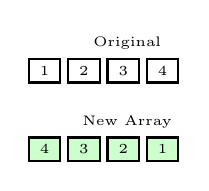
\begin{tikzpicture}[scale=0.5]
        \node at (2.5,3) {\tiny Original};
        \foreach \i/\val in {0/1, 1/2, 2/3, 3/4} {
          \draw[thick] (\i*1,2) rectangle (\i*1+0.8,2.6);
          \node at (\i*1+0.4,2.3) {\tiny\val};
        }

        \node at (2.5,1) {\tiny New Array};
        \foreach \i/\val in {0/4, 1/3, 2/2, 3/1} {
          \draw[thick, fill=green!20] (\i*1,0) rectangle (\i*1+0.8,0.6);
          \node at (\i*1+0.4,0.3) {\tiny\val};
        }
      \end{tikzpicture}
    \end{column}
    \begin{column}{0.48\textwidth}
      \begin{block}{In-place Algorithm}
        \textbf{Less Space, More Complex}
        \begin{lstlisting}[language=Python,basicstyle=\small\ttfamily]
def reverse_inplace(arr):
    left, right = 0, len(arr)-1
    while left < right:
        temp = arr[left]
        arr[left] = arr[right]
        arr[right] = temp
        left += 1
        right -= 1

# Modifies original
# Space: O(1)
        \end{lstlisting}
      \end{block}

      \vspace{0.3cm}

      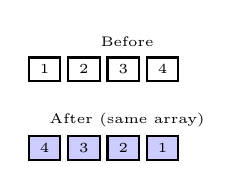
\begin{tikzpicture}[scale=0.5]
        \node at (2.5,3) {\tiny Before};
        \foreach \i/\val in {0/1, 1/2, 2/3, 3/4} {
          \draw[thick] (\i*1,2) rectangle (\i*1+0.8,2.6);
          \node at (\i*1+0.4,2.3) {\tiny\val};
        }

        \node at (2.5,1) {\tiny After (same array)};
        \foreach \i/\val in {0/4, 1/3, 2/2, 3/1} {
          \draw[thick, fill=blue!20] (\i*1,0) rectangle (\i*1+0.8,0.6);
          \node at (\i*1+0.4,0.3) {\tiny\val};
        }
      \end{tikzpicture}
    \end{column}
  \end{columns}
\end{frame}

\begin{frame}{When to Choose What?}
  \begin{columns}
    \begin{column}{0.48\textwidth}
      \begin{block}{Optimize for Time When:}
        \begin{itemize}
          \item Dealing with large datasets
          \item User experience matters
          \item Memory is abundant
          \item Real-time requirements
          \item Interactive applications
        \end{itemize}
      \end{block}

      \vspace{0.3cm}

      \begin{exampleblock}{Examples}
        \begin{itemize}
          \item Web servers (caching)
          \item Video games
          \item Trading systems
          \item Search engines
        \end{itemize}
      \end{exampleblock}
    \end{column}
    \begin{column}{0.48\textwidth}
      \begin{block}{Optimize for Space When:}
        \begin{itemize}
          \item Memory is limited
          \item Embedded systems
          \item Mobile devices
          \item Data too large for RAM
          \item Resource-constrained devices
        \end{itemize}
      \end{block}

      \vspace{0.3cm}

      \begin{exampleblock}{Examples}
        \begin{itemize}
          \item IoT devices
          \item Microcontrollers
          \item Big data processing
          \item Satellite systems
        \end{itemize}
      \end{exampleblock}
    \end{column}
  \end{columns}
\end{frame}

%----------------------------------------------------------------------------------------
%    BIG-O NOTATION
%----------------------------------------------------------------------------------------
\section{Asymptotic Analysis \& Big-O}

\begin{frame}{Why Asymptotic Analysis?}
  \begin{block}{The Problem with Exact Counts}
    Actual runtime depends on:
    \begin{itemize}
      \item Hardware (CPU speed, memory)
      \item Programming language
      \item Compiler optimizations
      \item Current system load
    \end{itemize}
  \end{block}

  \vspace{0.3cm}

  \begin{block}{The Solution: Asymptotic Analysis}
    Focus on \textbf{growth rate} as input size approaches infinity
    \begin{itemize}
      \item Hardware-independent
      \item Language-independent
      \item Describes \textbf{scalability}
      \item Constants become insignificant with large n
    \end{itemize}
  \end{block}

  \vspace{0.3cm}

  \begin{alertblock}{Big-O Notation}
    Describes the \textbf{upper bound} of an algorithm's growth rate (worst-case scenario)
  \end{alertblock}
\end{frame}

\begin{frame}{Common Big-O Classes}
  \begin{center}
    \begin{tabular}{l|l|l|c}
      \toprule
      \textbf{Notation} & \textbf{Name} & \textbf{Example} & \textbf{n=100} \\
      \midrule
      O(1) & Constant & Array access, hash lookup & 1 \\
      O(log n) & Logarithmic & Binary search & $\approx$ 7 \\
      O(n) & Linear & Linear search, scan & 100 \\
      O(n log n) & Linearithmic & Merge sort, quicksort & $\approx$ 664 \\
      O(n²) & Quadratic & Nested loops, bubble sort & 10,000 \\
      O(n³) & Cubic & Triple nested loops & 1,000,000 \\
      O(2$^n$) & Exponential & Recursive fibonacci & $\approx 10^{30}$ \\
      O(n!) & Factorial & All permutations & $\approx 10^{157}$ \\
      \bottomrule
    \end{tabular}
  \end{center}

  \vspace{0.5cm}

  \begin{alertblock}{Visual Scale}
    For n = 100, O(2$^n$) is \textbf{universe-ending}! Exponential growth is catastrophic.
  \end{alertblock}
\end{frame}

\begin{frame}{Big-O Growth Visualization}
  \begin{center}
    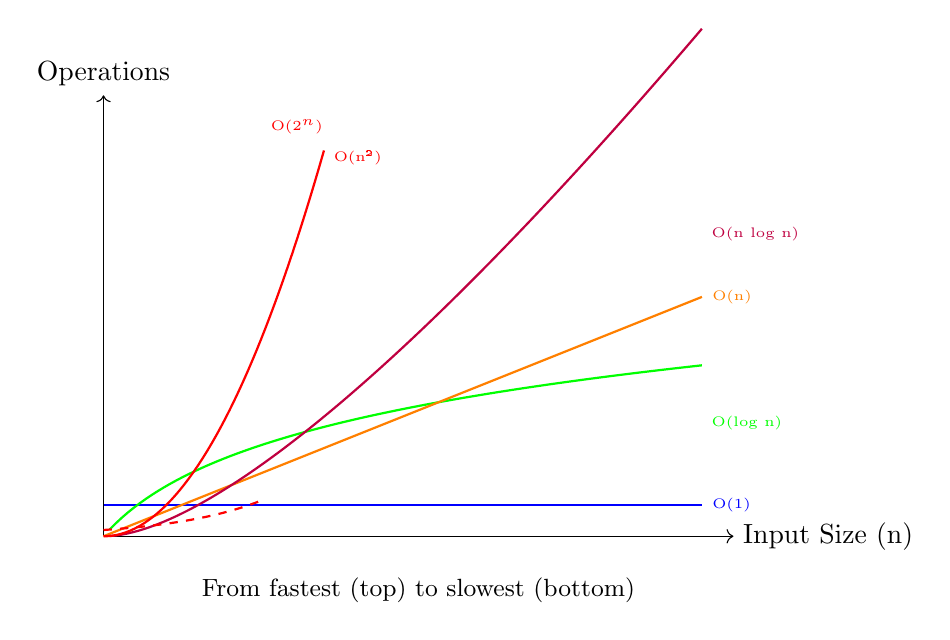
\begin{tikzpicture}[scale=0.8]
      \draw[->] (0,0) -- (10,0) node[right] {Input Size (n)};
      \draw[->] (0,0) -- (0,7) node[above] {Operations};

      % O(1)
      \draw[thick, blue] (0,0.5) -- (9.5,0.5) node[right] {\tiny O(1)};

      % O(log n)
      \draw[thick, green] plot[domain=0.1:9.5, samples=100] (\x, {0.8*ln(\x+1)/ln(2)});
      \node[green, right] at (9.5,1.8) {\tiny O(log n)};

      % O(n)
      \draw[thick, orange] (0,0) -- (9.5,3.8) node[right] {\tiny O(n)};

      % O(n log n)
      \draw[thick, purple] plot[domain=0.1:9.5, samples=100] (\x, {0.5*\x*ln(\x+1)/ln(2)/2});
      \node[purple, right] at (9.5,4.8) {\tiny O(n log n)};

      % O(n^2)
      \draw[thick, red] plot[domain=0:3.5, samples=50] (\x, {\x*\x/2});
      \node[red, right] at (3.5,6) {\tiny O(n²)};

      % O(2^n) - too steep to show fully
      \draw[thick, red, dashed] plot[domain=0:2.5, samples=30] (\x, {0.1*2^\x});
      \node[red, right] at (2.5,6.5) {\tiny O(2$^n$)};

      \node[below] at (5,-0.5) {\small From fastest (top) to slowest (bottom)};
    \end{tikzpicture}
  \end{center}

  \begin{block}{Key Observation}
    As n increases, differences between complexities become dramatic
  \end{block}
\end{frame}

\begin{frame}{Big-O Rules}
  \begin{columns}
    \begin{column}{0.48\textwidth}
      \begin{block}{Rule 1: Drop Constants}
        O(2n) $\rightarrow$ O(n) \\
        O(100) $\rightarrow$ O(1) \\
        O(n/2) $\rightarrow$ O(n)

        \vspace{0.2cm}

        \textbf{Why?} Constants don't affect growth rate
      \end{block}

      \vspace{0.3cm}

      \begin{block}{Rule 2: Drop Lower-Order Terms}
        O($n^2$ + n) $\rightarrow$ O($n^2$) \\
        O($n^2$ + 100*n + 50) $\rightarrow$ O($n^2$) \\
        O($n^3$ + $n^2$ + n) $\rightarrow$ O($n^3$)

        \vspace{0.2cm}

        \textbf{Why?} Highest order dominates for large n
      \end{block}
    \end{column}
    \begin{column}{0.48\textwidth}
      \begin{block}{Rule 3: Different Variables}
        Two inputs? Use different variables!
        \vspace{0.2cm}
        Sequential: O(a + b) \\
        Nested: O(a * b)
%         \begin{lstlisting}[language=Python,basicstyle=\tiny\ttfamily]
% % for i in arr1:  # n iterations
% %     process(i)
% % for j in arr2:  # m iterations
% %     process(j)
% % # O(n + m)
% % for i in arr1:  # n iterations
% %     for j in arr2:  # m iterations
% %         process(i, j)
% % # O(n * m)
%         \end{lstlisting}
      \end{block}
    \end{column}
  \end{columns}

  \vspace{0.3cm}

  \begin{alertblock}{Rule 4: Worst Case}
    Big-O describes the \textbf{worst-case} scenario by default
  \end{alertblock}
\end{frame}

\begin{frame}[fragile]{Big-O Examples}
  \begin{columns}
    \begin{column}{0.48\textwidth}
      \begin{exampleblock}{O(1) - Constant}
        \begin{lstlisting}[language=Python,basicstyle=\tiny\ttfamily]
def get_first(arr):
    return arr[0]
# Always 1 operation
        \end{lstlisting}
      \end{exampleblock}

      \begin{exampleblock}{O(n) - Linear}
        \begin{lstlisting}[language=Python,basicstyle=\tiny\ttfamily]
def find_max(arr):
    max_val = arr[0]
    for num in arr:  # n iterations
        if num > max_val:
            max_val = num
    return max_val
        \end{lstlisting}
      \end{exampleblock}

      \begin{exampleblock}{O(n²) - Quadratic}
        \begin{lstlisting}[language=Python,basicstyle=\tiny\ttfamily]
def bubble_sort(arr):
    n = len(arr)
    for i in range(n):      # n times
        for j in range(n-1): # n times
            if arr[j] > arr[j+1]:
                arr[j], arr[j+1] = \
                    arr[j+1], arr[j]
        \end{lstlisting}
      \end{exampleblock}
    \end{column}
    \begin{column}{0.48\textwidth}
      \begin{exampleblock}{O(log n) - Logarithmic}
        \begin{lstlisting}[language=Python,basicstyle=\tiny\ttfamily]
def binary_search(arr, target):
    left, right = 0, len(arr) - 1
    while left <= right:
        mid = (left + right) // 2
        if arr[mid] == target:
            return mid
        elif arr[mid] < target:
            left = mid + 1
        else:
            right = mid - 1
        # Halves search space each time!
    return -1
        \end{lstlisting}
      \end{exampleblock}

      \begin{exampleblock}{O(n log n) - Linearithmic}
        \begin{lstlisting}[language=Python,basicstyle=\tiny\ttfamily]
def merge_sort(arr):
    if len(arr) <= 1:
        return arr
    mid = len(arr) // 2
    left = merge_sort(arr[:mid])
    right = merge_sort(arr[mid:])
    return merge(left, right)
# log n divisions, n work per level
        \end{lstlisting}
      \end{exampleblock}
    \end{column}
  \end{columns}
\end{frame}

%----------------------------------------------------------------------------------------
%    COMMON OPERATIONS
%----------------------------------------------------------------------------------------
\section{Big-O of Common Operations}

% \begin{frame}{Arrays (Lists)}
%   \begin{center}
%     \begin{tabular}{l|c|p{5cm}}
%       \toprule
%       \textbf{Operation} & \textbf{Time} & \textbf{Notes} \\
%       \midrule
%       Access by index & O(1) & Direct memory access \\
%       Search (unsorted) & O(n) & Must check each element \\
%       Search (sorted) & O(log n) & Can use binary search \\
%       Insert at end & O(1) amortized & May need to resize \\
%       Insert at beginning & O(n) & Must shift all elements \\
%       Delete at end & O(1) & Simple removal \\
%       Delete at beginning & O(n) & Must shift all elements \\
%       \bottomrule
%     \end{tabular}
%   \end{center}

%   \vspace{0.5cm}

%   \begin{columns}
%     \begin{column}{0.48\textwidth}
%       \begin{block}{Strengths}
%         \begin{itemize}
%           \item[$\checkmark$] Fast random access
%           \item[$\checkmark$] Cache-friendly
%           \item[$\checkmark$] Simple to use
%         \end{itemize}
%       \end{block}
%     \end{column}
%     \begin{column}{0.48\textwidth}
%       \begin{block}{Weaknesses}
%         \begin{itemize}
%           \item[$\times$] Slow insert/delete in middle
%           \item[$\times$] Fixed/resize overhead
%           \item[$\times$] Wasted space if sparse
%         \end{itemize}
%       \end{block}
%     \end{column}
%   \end{columns}
% \end{frame}

% \begin{frame}{Other Data Structures}
%   \begin{center}
%     \small
%     \begin{tabular}{l|l|c|c|p{3cm}}
%       \toprule
%       \textbf{Structure} & \textbf{Operation} & \textbf{Average} & \textbf{Worst} & \textbf{Notes} \\
%       \midrule
%       \multirow{3}{*}{Linked List}
%         & Access & O(n) & O(n) & Must traverse \\
%         & Insert (front) & O(1) & O(1) & Update head \\
%         & Delete (front) & O(1) & O(1) & Update head \\
%       \midrule
%       \multirow{3}{*}{Hash Table}
%         & Search & O(1) & O(n) & Collisions \\
%         & Insert & O(1) & O(n) & Rehashing \\
%         & Delete & O(1) & O(n) & Collisions \\
%       \midrule
%       \multirow{3}{*}{BST (Balanced)}
%         & Search & O(log n) & O(n) & Unbalanced worst \\
%         & Insert & O(log n) & O(n) & Unbalanced worst \\
%         & Delete & O(log n) & O(n) & Unbalanced worst \\
%       \midrule
%       \multirow{2}{*}{Stack/Queue}
%         & Push/Enqueue & O(1) & O(1) & Top/rear only \\
%         & Pop/Dequeue & O(1) & O(1) & Top/front only \\
%       \midrule
%       \multirow{3}{*}{Heap}
%         & Find min/max & O(1) & O(1) & Root element \\
%         & Insert & O(log n) & O(log n) & Bubble up \\
%         & Delete min/max & O(log n) & O(log n) & Bubble down \\
%       \bottomrule
%     \end{tabular}
%   \end{center}
% \end{frame}

\begin{frame}{Sorting Algorithms Comparison}
  \begin{center}
    \begin{tabular}{l|c|c|c|c}
      \toprule
      \textbf{Algorithm} & \textbf{Average} & \textbf{Worst} & \textbf{Space} & \textbf{Stable?} \\
      \midrule
      Quick Sort & O(n log n) & O(n²) & O(log n) & No \\
      Merge Sort & O(n log n) & O(n log n) & O(n) & Yes \\
      Heap Sort & O(n log n) & O(n log n) & O(1) & No \\
      Bubble Sort & O(n²) & O(n²) & O(1) & Yes \\
      Insertion Sort & O(n²) & O(n²) & O(1) & Yes \\
      \bottomrule
    \end{tabular}
  \end{center}

  \vspace{0.5cm}

  \begin{block}{Quick Selection Guide}
    \begin{itemize}
      \item Need \textbf{fast random access}? $\rightarrow$ Arrays
      \item Need \textbf{fast insertion/deletion at beginning}? $\rightarrow$ Linked lists
      \item Need \textbf{fast key-value lookup}? $\rightarrow$ Hash tables
      \item Need \textbf{sorted data with fast operations}? $\rightarrow$ Balanced BSTs
      \item Need \textbf{LIFO access}? $\rightarrow$ Stacks
      \item Need \textbf{FIFO access}? $\rightarrow$ Queues
      \item Need \textbf{min/max quickly}? $\rightarrow$ Heaps
    \end{itemize}
  \end{block}
\end{frame}

%----------------------------------------------------------------------------------------
%    CHOOSING STRUCTURES
%----------------------------------------------------------------------------------------
\section{When to Choose a Structure}

\begin{frame}{Decision Framework}
  \begin{block}{Questions to Ask}
    \begin{enumerate}
      \item \textbf{What operations will be most frequent?}
        \begin{itemize}
          \item Lookups? $\rightarrow$ Hash table or BST
          \item Insertions/deletions? $\rightarrow$ Linked list or balanced tree
          \item Processing in order? $\rightarrow$ Queue
          \item Need to undo? $\rightarrow$ Stack
        \end{itemize}

      \item \textbf{Do you need ordered data?}
        \begin{itemize}
          \item Yes, sorted $\rightarrow$ BST, sorted array
          \item Yes, insertion order $\rightarrow$ Array, linked list
          \item No $\rightarrow$ Hash table (fastest)
        \end{itemize}

      \item \textbf{Do you know the size in advance?}
        \begin{itemize}
          \item Yes, fixed $\rightarrow$ Array
          \item No, dynamic $\rightarrow$ Linked list, dynamic array, hash table
        \end{itemize}

      \item \textbf{What are your constraints?}
        \begin{itemize}
          \item Limited memory $\rightarrow$ Space-efficient structures
          \item Need speed $\rightarrow$ Time-efficient structures
        \end{itemize}
    \end{enumerate}
  \end{block}
\end{frame}

\begin{frame}[fragile]{Real-World Scenario 1: Phone Book}
  \begin{columns}
    \begin{column}{0.48\textwidth}
      \begin{block}{Requirements}
        \begin{itemize}
          \item Fast lookup by name
          \item Alphabetical order useful
          \item Operations:
            \begin{itemize}
              \item Search (frequent)
              \item Insert (rare)
              \item Delete (rare)
            \end{itemize}
        \end{itemize}
      \end{block}

      \vspace{0.3cm}

      \begin{alertblock}{Decision}
        \textbf{Hash table} for O(1) lookup \\
        or \textbf{BST} for O(log n) with ordering
      \end{alertblock}
    \end{column}
    \begin{column}{0.48\textwidth}
      \begin{exampleblock}{Implementation}
        \begin{lstlisting}[language=Python,basicstyle=\small\ttfamily]
# Using hash table
phone_book = {
    "Alice": "555-1234",
    "Bob": "555-5678"
}

# O(1) lookup
number = phone_book["Alice"]
        \end{lstlisting}
      \end{exampleblock}
    \end{column}
  \end{columns}
\end{frame}

\begin{frame}[fragile]{Real-World Scenario 2: Browser History}
  \begin{columns}
    \begin{column}{0.48\textwidth}
      \begin{block}{Requirements}
        \begin{itemize}
          \item Recent pages accessed frequently
          \item Navigate back and forward
          \item Operations:
            \begin{itemize}
              \item Push new page
              \item Go back (pop)
              \item Go forward (pop)
            \end{itemize}
        \end{itemize}
      \end{block}

      \vspace{0.3cm}

      \begin{alertblock}{Decision}
        \textbf{Two stacks:} \\
        - Back stack \\
        - Forward stack
      \end{alertblock}
    \end{column}
    \begin{column}{0.48\textwidth}
      \begin{exampleblock}{Implementation}
        \begin{lstlisting}[language=Python,basicstyle=\tiny\ttfamily]
back_stack = []
forward_stack = []

def visit_page(url):
    back_stack.append(current_page)
    forward_stack.clear()
    current_page = url

def go_back():
    if back_stack:
        forward_stack.append(current_page)
        current_page = back_stack.pop()

def go_forward():
    if forward_stack:
        back_stack.append(current_page)
        current_page = forward_stack.pop()
        \end{lstlisting}
      \end{exampleblock}
    \end{column}
  \end{columns}
\end{frame}

\begin{frame}[fragile]{Real-World Scenario 3: Print Queue}
  \begin{columns}
    \begin{column}{0.48\textwidth}
      \begin{block}{Requirements}
        \begin{itemize}
          \item First document submitted prints first
          \item Operations:
            \begin{itemize}
              \item Add to queue (frequent)
              \item Remove from queue (frequent)
            \end{itemize}
          \item FIFO behavior essential
        \end{itemize}
      \end{block}

      \vspace{0.3cm}

      \begin{alertblock}{Decision}
        \textbf{Queue} \\
        (First In, First Out)
      \end{alertblock}
    \end{column}
    \begin{column}{0.48\textwidth}
      \begin{exampleblock}{Implementation}
        \begin{lstlisting}[language=Python,basicstyle=\small\ttfamily]
from collections import deque

print_queue = deque()

# Enqueue documents
print_queue.append("doc1.pdf")
print_queue.append("doc2.pdf")
print_queue.append("doc3.pdf")

# Dequeue - FIFO
current_job = print_queue.popleft()
# "doc1.pdf" prints first
        \end{lstlisting}
      \end{exampleblock}
    \end{column}
  \end{columns}
\end{frame}

\begin{frame}{Common Pitfalls}
  \begin{alertblock}{What NOT to Do}
    \begin{itemize}
      \item[$\times$] Using lists for frequent lookups \\
            {\small (O(n) instead of O(1) with hash table)}
      \item[$\times$] Using arrays when size is unknown \\
            {\small (Costly resizing)}
      \item[$\times$] Using BST when order doesn't matter \\
            {\small (Hash table is faster)}
      \item[$\times$] Using recursive structures without considering stack overflow \\
            {\small (Deep recursion can crash)}
    \end{itemize}
  \end{alertblock}

  \vspace{0.5cm}

  \begin{block}{General Guidelines}
    \begin{itemize}
      \item \textbf{Default to hash tables} for key-value storage (most versatile)
      \item \textbf{Use arrays} when you need index-based access
      \item \textbf{Use linked lists} when you have many insertions/deletions
      \item \textbf{Use trees} when you need both ordering and fast operations
      \item \textbf{Use specialized structures} when they match your access pattern
    \end{itemize}
  \end{block}
\end{frame}

%----------------------------------------------------------------------------------------
%    ADTs
%----------------------------------------------------------------------------------------
\section{Abstraction and ADTs}

\begin{frame}{Abstract Data Types (ADT)}
  \begin{definition}
    An \textbf{ADT} defines a data type by its \textbf{behavior} (operations) rather than its implementation. It specifies \textbf{what} operations can be performed, not \textbf{how}.
  \end{definition}

  \vspace{0.5cm}

  \begin{block}{Key Principle}
    Separate the \textbf{interface} (what operations are available) from the \textbf{implementation} (how they work internally)
  \end{block}

  \vspace{0.3cm}

  \begin{columns}
    \begin{column}{0.48\textwidth}
      \begin{exampleblock}{Benefits}
        \begin{enumerate}
          \item \textbf{Flexibility} \\
                Change implementation without affecting users
          \item \textbf{Simplicity} \\
                Hide internal complexity
          \item \textbf{Reusability} \\
                Same interface, different implementations
          \item \textbf{Maintainability} \\
                Easier to update and fix
        \end{enumerate}
      \end{exampleblock}
    \end{column}
    \begin{column}{0.48\textwidth}
      \begin{exampleblock}{Real-World Analogy}
        \textbf{ADT = Car Interface}
        \begin{itemize}
          \item Steering wheel
          \item Gas pedal
          \item Brake
        \end{itemize}

        \textbf{Implementation}
        \begin{itemize}
          \item Electric car
          \item Gas car
        \end{itemize}

        Same interface, different internals!
      \end{exampleblock}
    \end{column}
  \end{columns}
\end{frame}

\begin{frame}[fragile]{ADT Example: Stack}
  \begin{columns}
    \begin{column}{0.48\textwidth}
      \begin{block}{Stack ADT Interface}
        \begin{lstlisting}[language=Python,basicstyle=\tiny\ttfamily]
class StackADT:
    def push(self, item): pass
    def pop(self): pass
    def peek(self): pass
    def is_empty(self): pass

# Behavior: LIFO
# (Last In, First Out)
        \end{lstlisting}
      \end{block}

      \vspace{0.3cm}

      \begin{exampleblock}{Implementation 1: Array}
        \begin{lstlisting}[language=Python,basicstyle=\tiny\ttfamily]
class ArrayStack(StackADT):
    def __init__(self):
        self._data = []

    def push(self, item):
        self._data.append(item)

    def pop(self):
        return self._data.pop()

    def peek(self):
        return self._data[-1]

    def is_empty(self):
        return len(self._data) == 0
        \end{lstlisting}
      \end{exampleblock}
    \end{column}
    \begin{column}{0.48\textwidth}
      \begin{exampleblock}{Implementation 2: Linked List}
        \begin{lstlisting}[language=Python,basicstyle=\tiny\ttfamily]
class LinkedStack(StackADT):
    def __init__(self):
        self._head = None
        self._size = 0

    def push(self, item):
        new_node = Node(item, self._head)
        self._head = new_node
        self._size += 1

    def pop(self):
        if not self._head:
            raise IndexError("empty")
        value = self._head.value
        self._head = self._head.next
        self._size -= 1
        return value

    def peek(self):
        if not self._head:
            raise IndexError("empty")
        return self._head.value

    def is_empty(self):
        return self._head is None
        \end{lstlisting}
      \end{exampleblock}
    \end{column}
  \end{columns}

  \vspace{0.3cm}

  \begin{center}
    \textbf{Same interface, different implementations!} Users don't need to know which one is being used.
  \end{center}
\end{frame}

\begin{frame}{ADT Hierarchy}
  \begin{center}
    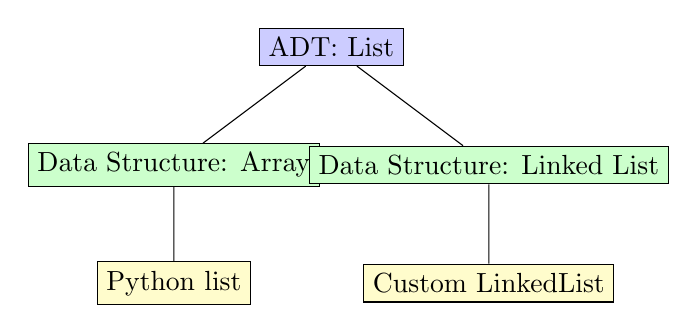
\begin{tikzpicture}[
      level 1/.style={sibling distance=4cm, level distance=1.5cm},
      level 2/.style={sibling distance=2cm, level distance=1.5cm}
    ]
      \node[draw, rectangle, fill=blue!20] {ADT: List}
        child {node[draw, rectangle, fill=green!20] {Data Structure: Array}
          child {node[draw, rectangle, fill=yellow!20] {Python list}}
        }
        child {node[draw, rectangle, fill=green!20] {Data Structure: Linked List}
          child {node[draw, rectangle, fill=yellow!20] {Custom LinkedList}}
        };
    \end{tikzpicture}
  \end{center}

  \vspace{0.5cm}

  \begin{block}{Three Levels}
    \begin{itemize}
      \item \textbf{ADT} (Abstract): The concept/interface (e.g., "List")
      \item \textbf{Data Structure} (Logical): How data is organized (e.g., "Array" or "Linked List")
      \item \textbf{Implementation} (Physical): Actual code in a programming language
    \end{itemize}
  \end{block}
\end{frame}

\begin{frame}[fragile]{Encapsulation in ADTs}
  \begin{columns}
    \begin{column}{0.48\textwidth}
      \begin{exampleblock}{Good: Hidden Implementation}
        \begin{lstlisting}[language=Python,basicstyle=\tiny\ttfamily]
class Stack:
    def __init__(self):
        self._data = []  # Private

    def push(self, item):
        self._data.append(item)

    def pop(self):
        return self._data.pop()

# Users can't access _data directly
# Implementation can change!
        \end{lstlisting}

        \vspace{0.2cm}

        {\color{green!70!black}$\checkmark$} Implementation hidden \\
        {\color{green!70!black}$\checkmark$} Can swap to linked list easily \\
        {\color{green!70!black}$\checkmark$} Users can't break invariants
      \end{exampleblock}
    \end{column}
    \begin{column}{0.48\textwidth}
      \begin{alertblock}{Bad: Exposed Implementation}
        \begin{lstlisting}[language=Python,basicstyle=\tiny\ttfamily]
class BadStack:
    def __init__(self):
        self.data = []  # Public!

    def push(self, item):
        self.data.append(item)

    def pop(self):
        return self.data.pop()

# Problem:
stack = BadStack()
stack.data = "oops!"  # Breaks it!
stack.data.clear()     # Ruins stack!
        \end{lstlisting}

        \vspace{0.2cm}

        {\color{red}$\times$} Implementation exposed \\
        {\color{red}$\times$} Users can break the stack \\
        {\color{red}$\times$} Hard to change implementation
      \end{alertblock}
    \end{column}
  \end{columns}
\end{frame}

%----------------------------------------------------------------------------------------
%    SUMMARY
%----------------------------------------------------------------------------------------
\section{Summary}

\begin{frame}{Key Takeaways}
  \begin{block}{1. Data Structures Matter}
    \begin{itemize}
      \item Right structure = milliseconds, Wrong structure = hours
      \item Choose based on most frequent operations
      \item Understand time vs space trade-offs
    \end{itemize}
  \end{block}

  \begin{block}{2. Big-O Analysis}
    \begin{itemize}
      \item Describes growth rate, not exact time
      \item Focus on scalability for large inputs
      \item Remember: O(1) < O(log n) < O(n) < O(n log n) < O(n²) < O(2$^n$)
      \item Drop constants and lower-order terms
    \end{itemize}
  \end{block}

  \begin{block}{3. Common Operations}
    \begin{itemize}
      \item Arrays: O(1) access, O(n) insert/delete in middle
      \item Hash tables: O(1) average lookup/insert/delete
      \item BSTs: O(log n) for balanced trees
      \item Stacks/Queues: O(1) push/pop
    \end{itemize}
  \end{block}
\end{frame}

\begin{frame}{Key Takeaways (continued)}
  \begin{block}{4. Choosing Structures}
    \begin{itemize}
      \item Ask: What operations are most frequent?
      \item Ask: Do you need ordering?
      \item Ask: What are your constraints (time/space)?
      \item Default to hash tables for key-value storage
      \item Use specialized structures when they match your pattern
    \end{itemize}
  \end{block}

  \begin{block}{5. Abstract Data Types}
    \begin{itemize}
      \item Separate interface from implementation
      \item Hide internal details (encapsulation)
      \item Makes code flexible and maintainable
      \item Same interface, multiple implementations
    \end{itemize}
  \end{block}

  \vspace{0.3cm}

  \begin{alertblock}{Next Steps}
    Study specific data structures in depth: Arrays, Linked Lists, Stacks, Queues, Trees, Graphs, Hash Tables, and more!
  \end{alertblock}
\end{frame}

\begin{frame}[plain]
  \begin{center}
    {\Huge Thank You!}

    \vspace{1cm}

    {\large Questions?}

    \vspace{1cm}

    \textit{``Choosing the right data structure \\
    is half the battle in algorithm design.''}
  \end{center}
\end{frame}

\end{document}
